\chapter{Framework}

Lo sviluppo del software QSapecNG si è appoggiato a framework esistenti, in grado di offrire tutto ciò che fosse necessario per snellire, semplificare ed ottimizzare la procedura di scrittura del codice. In particolare, data la crucialità del ruolo ricoperto dall'algoritmo per la ricerca degli alberi di copertura comuni su due grafi, era necessario appoggiarsi ad una libreria che mettesse a disposizione allo stesso tempo strutture dati maneggevoli per la definizione di grafi e modelli flessibili per la stesura di algoritmi che operassero su tali grafi. Non meno importante si è dimostrata anche la necessità di disporre di una libreria di componenti grafici capace di dimostrarsi completa sotto tutti gli aspetti e in grado di rendere veloce lo sviluppo senza appesantirlo in un crescendo di complessità. Non bisogna poi tralasciare tutti quegli aspetti che all'utente finale possono apparire come di corredo o addirittura essere celati ma che, nelle fasi di sviluppo, possono presentarsi come veri e propri ostacoli e per questo motivo devono essere affrontati con i giusti mezzi.

Per tutti i motivi sopra brevemente accennati e per molti altri che sarebbe tedioso elencare, la scelta è ricaduta su due pietre miliari del mondo C++, ovvero:
\begin{itemize}
 \item La libreria di librerie C++: Boost C++ Libraries \cite{Boost}.
 \item Il framework Qt \cite{Qt}, componenti per lo sviluppo di applicativi multi-piattaforma grafici e non.
\end{itemize}
Grazie ad esse il software QSapecNG si è sviluppato in modo pulito e coerente, con un po' di oculatezza nella scrittura è risultato essere interamente portabile e pertanto si presenta come un applicativo multi-piattaforma per il disegno, la risoluzione simbolica e l'analisi del comportamento di circuiti elettrici.\\
Senza dilungarsi troppo, è necessario quindi effettuare una veloce panoramica dei due colossi utilizzati.


\section{Boost C++ Libraries}
Da Herb Sutter e Andrei Alexandrescu viene definita \cite{CppCodStd} come:
\begin{quote}
 ... one of the most highly regarded and expertly designed C++ library projects in the world.
\end{quote}

Scott Meyers avanza un consiglio in proposito \cite{EffectiveCpp} fra le cose da fare per i novizi del pianeta C++:
\begin{quote}
 Item $55$: Familiarize yourself with Boost.
\end{quote}

Bjarne Stroustrup, una delle menti che stanno dietro alla definizione del linguaggio C++ e autore del libro \cite{Stroustrup} considerato la guida introduttiva di base per chi vuole avvicinarsi al linguaggio, alla domanda su cosa pensi di Boost risponde:
\begin{quote}
Boost is a large and expanding collection of libraries designed to work well with the ISO C++ standard library. It contains many extremely useful and well-engineered libraries, such as asio, filesystem, regex, and thread (apologies for not trying to identify more useful libraries; there are just too many). One library, $TR1$, contains a good approximation of new C++$0x$ standard library components.

The Boost libraries
\begin{itemize}
 \item Have tests suites.
 \item Have documentation.
 \item  Have been tested on multiple systems.
 \item Are peer-reviewed.
\end{itemize}

[...]

That said, it is usually a really dumb idea to go and reinvent a wheel that boost already offers.
\end{quote}
Mentre in un suo articolo \cite{StroustrupCpp} afferma:
\begin{quote}
 The obvious solution for most programmers is to use a library that provides an elegant and efficient platform independent to needed services. Examples are BOOST...
\end{quote}

Boost C++\graffito{Boost C++ è spesso usata come ausilio alla programmazione, per sopperire a tutte le carenze della libreria standard (plausibili, motivate o meno)}, quella che si potrebbe definire una libreria di librerie risulta quindi essere apprezzata e ben vista anche dai maggiori esponenti dell'ambiente C++, al di là del suo essere equilibratamente complicata tanto per i novizi quanto per gli esperti. Sviluppata in maniera modulare e con componenti strettamente legati l'un l'altro (croce e delizia di chi si avvicina per la prima volta), offre alti standard di qualità e un ventaglio di soluzioni per le più disparate necessità. Si articola attraverso tecniche di programmazione generica, l'uso di \textit{concept} e \textit{traits} e molto altro ancora, mostrandosi in grado di rendere estremamente flessibile lo sviluppo e l'utilizzo delle diverse librerie, alzando soltanto di poco la curva di apprendimento e mettendo a disposizione in molti casi soluzioni semplici per chi preferisce non scoprire cosa vi è dietro.

Le librerie Boost C++ sono di fatto, volenti o nolenti, una realtà sempre più integrata negli standard C++ che da essa attingono e ad essa forniscono gli strumenti per migliorarsi sempre più. Una realtà che, inevitabilmente, deve essere presa in considerazione e spesso offre la risposte a gran parte delle problematiche incontrate nello sviluppo.

\paragraph{BGL: The Boost Graph Library}
Sarebbe interessante, in questo frangente, discutere di tutte le librerie presenti in Boost e utilizzate anche nella stesura del codice di QSapecNG (quali \textit{Property Tree}, \textit{Property Map}, \textit{Foreach}, \textit{Bimap} e via dicendo), eppure un tale argomento risulterebbe forse fin troppo ampio e mal digerito da chiunque non sia appassionato di programmazione e interessato ai dettagli del software.\\
Ciò nonostante bisogna obbligatoriamente soffermarsi almeno su una di esse, poiché si sono sviluppati algoritmi conformi alle direttive proposte che vanno a collocarsi direttamente nella panoramica offerta da Boost. Un'analisi dettagliata di tali algoritmi è riportata nei capitoli che seguono mentre una breve introduzione e descrizione della libreria interessata avrà qui luogo.

In particolare la libreria in questione è la \textbf{BGL: Boost Graph Library} \cite{BGL}. Essa rappresenta una risposta alla necessità di strutture dati per la rappresentazione e gestione di grafi, oltre a fornire le basi per lo sviluppo di codice generico da applicare su tali strutture (nel caso specifico, atto ad individuare gli alberi di copertura comuni dati due grafi).\\
La BGL mette a disposizione interfacce, algoritmi e componenti generici nello stesso senso in cui risulta generica la \textbf{STL (Standard Template Library)} \cite{STL}. Come riportato dalla documentazione, la BGL è generica nei modi che seguono (parafrasando appunto il modello della STL):
\begin{itemize}
 \item Interoperabilità fra algoritmi e strutture dati: i grafi sono sviluppati su un concetto di interfaccia e nascondono la reale implementazione (sia essa in forma di lista di archi, matrice o lista di adiacenza), per cui gli algoritmi possono essere resi altrettanto generici e trattare svariati tipi di grafi, accedendo attraverso iteratori su archi e vertici in modo coerente ed omogeneo, senza preoccuparsi della forma e struttura sottoposta in ingresso.
 \item Estensione degli algoritmi: l'uso di oggetti conformi ad una interfaccia comune, detta visitatore, permette di estendere facilmente tutti quegli algoritmi a cui tali interfacce possono essere agganciate per dare luogo ad azioni specifiche in ben definiti punti chiave dell'esecuzione.
 \item Multi-parametrizzazione delle proprietà per vertici ed archi: senza scendere in dettagli, poiché l'argomento richiederebbe l'introduzione di un'ulteriore libreria presente in Boost (\textit{Property Map}), basti sapere che archi e vertici possono essere associati ad un numero arbitrario e indipendente di proprietà, ovvero informazioni che recano con loro durante l'esecuzione.
\end{itemize}

Inutile dire, poi, che è già disponibile un ampio parco di algoritmi base\graffito{Alcuni degli algoritmi presenti nella BGL sono la ricerca in profondità (depth first search, DFS), la ricerca in ampiezza (breadth first search, BFS), la ricerca del cammino minimo (algoritmo di Dijkstra), la ricerca delle componenti connesse e fortemente connesse, e molti altri ancora, alcuni dei quali proposti in più forme (ad esempio l'algoritmo per la ricerca degli alberi di copertura a peso minimo è presente nella versione di Kruskal e in quella di Prim)} da usare come tasselli per la costruzione di funzioni più complesse, anch'esse presenti per quanto possibile. Bisogna dire che non è disponibile, forse a causa della specificità dell'argomento, un algoritmo per la ricerca di alberi di copertura comuni fra due grafi, il quale sarà presto e orgogliosamente proposto (proprio a seguito dello sviluppo nell'ottica di QSapecNG) per l'integrazione nella BGL, essendo anche questo uno dei risultati ottenuti durante il lavoro di tesi.


\section{Qt}

\begin{figure}
 \centering
 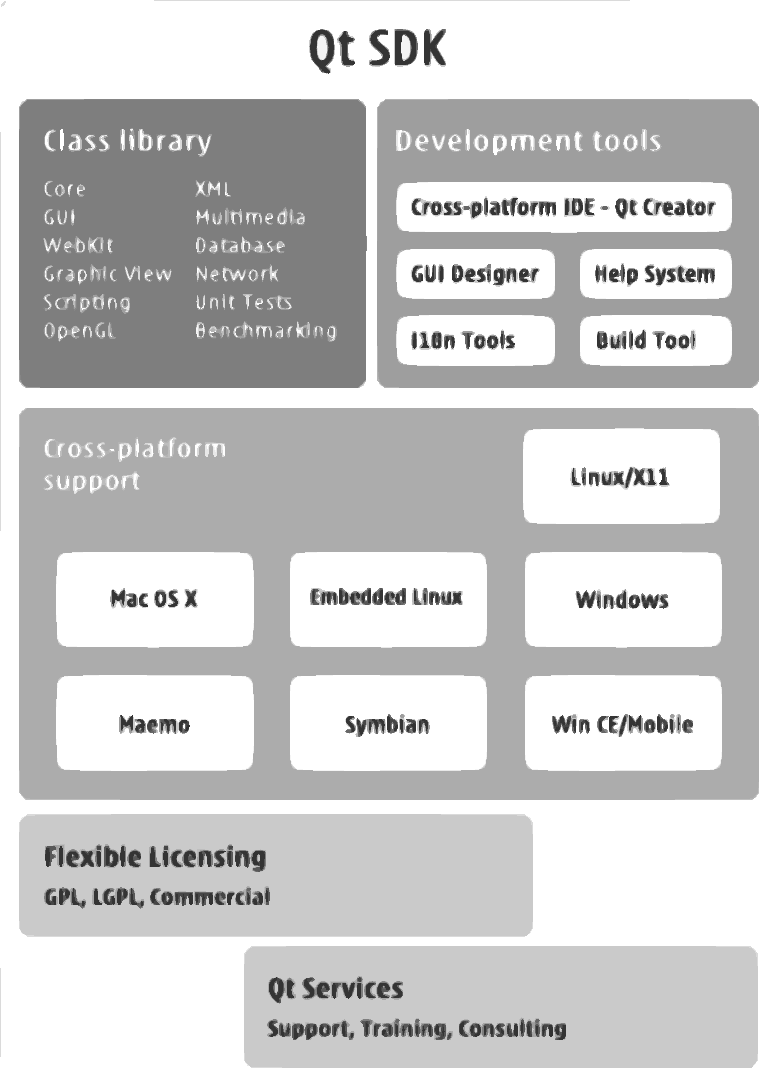
\includegraphics[scale=0.85]{immagini/qtschema.pdf}
 \caption{Qt SDK (schema)}
 \label{fig:qtschema}
\end{figure}

L'ambiente grafico (e non solo) ha sposato, invece, la proposta delle librerie Qt \cite{Qt}, un framework che non si limita ad offrire componenti per lo sviluppo di interfacce ma mette a disposizione molto di più, come ad esempio la possibilità di fornire soluzioni portabili, multi-threading, accessibili via web e tanto altro ancora.

Il Qt SDK (Software Development Kit), in figura \ref{fig:qtschema}, non rappresenta un semplice strumento o una libreria, è tutto ciò (o quasi) di cui uno sviluppatore può avere bisogno: librerie per lo sviluppo grafico, per il web, per il multimediale, per le basi dati e tanto altro a supporto delle necessità del programmatore; strumenti di sviluppo quali un IDE (Integrated Development Environment) multi-piattaforma, un ambiente per il disegno diretto delle interfacce, un sistema per la traduzione agile in lingue diverse rappresentano la punta dell'iceberg di offerte che accompagnano il framework; il modello di licenza, i servizi (gratuiti e non) messi a disposizione e il pieno supporto su un'ampia varietà di piattaforme sono il biglietto da visita del Qt SDK.

Anche in questa sede sarebbe forse interessante scendere dettagliatamente nel cuore del come e del cosa riguardanti lo sviluppo di un sistema CAD ma purtroppo, per ovvi motivi, questo non è realmente possibile. Più avanti saranno però trattati alcuni pattern che da Qt migrano direttamente nel processo di progettazione del software che fa uso di queste librerie, cercando di dare un'idea introduttiva sulle metodologie di programmazione utilizzate.
